%0       1         2         3         4         5         6         7         8
%2345678901234567890123456789012345678901234567890123456789012345678901234567890
%=======================================================================
\documentclass{book}
%=======================================================================


% INCLUDE DEVELOPMENT TEXT

\newcommand{\devel}[1]{\textbf{#1}}

% EXCLUDE DEVELOPMENT TEXT

% \newcommand{\devel}[1]{}


%=======================================================================
% Document layout
%=======================================================================

\setlength{\topmargin}{0.0in}
\setlength{\oddsidemargin}{0.0in}
\setlength{\evensidemargin}{0.0in}
\setlength{\textwidth}{6.0in}
\setlength{\textheight}{9.0in}

%=======================================================================
% Packages
%=======================================================================

\usepackage{wasysym}
\usepackage{epsfig}
\usepackage{url}

%=======================================================================
% Commands
%=======================================================================

\newcommand{\cello}{\textsf{Cello}}
\newcommand{\enzo}{\textsf{Enzo}}
\newcommand{\lcaperf}{\textsf{lcaperf}}
\newcommand{\lcatest}{\textsf{lcatest}}

\newcommand{\code}[1]{\textsf{#1}}

\newcommand{\note}[1]{\devel{\eighthnote\ \textit{#1} \\}}
\newcommand{\pargraph}[1]{\devel{\P\ \textbf{#1} \\}}

\newcommand{\todo}{\devel{$\circ$}}
\newcommand{\done}{\devel{$\bullet$}}
\newcommand{\halfdone}{\devel{\textcolor{gray}{$\bullet$}}}

\newcommand{\PROJECT}{\cello}

\newcommand{\TITLE}[3]{
\title{ {\huge \PROJECT\ #1}  \\ \vspace{0.1in}
     {\small Document Version: \textbf{#3}} \vspace{-0.1in}
    }
\author{      #2 \\
        Laboratory for Computational Astrophysics\\
        University of California, San Diego}
\maketitle}

%=======================================================================


%=======================================================================

\begin{document}

%=======================================================================
\TITLE{\cello\ UML Diagrams}{James Bordner}{$Rev: 383 $}
%=======================================================================

\tableofcontents

%=======================================================================
\title{Introduction} \label{s:intro}
%=======================================================================


%=======================================================================
\chapter{Use Case View}
%=======================================================================

%=======================================================================
\chapter{Design View}
%=======================================================================


%=======================================================================
\section{Disk}
%=======================================================================

Provides functions for writing and reading data to and from disk
storage

%=======================================================================
\section{Distribute}
%=======================================================================

Distribute (and dynamically redistribute) Tasks among nodes and
processes

%=======================================================================
\section{Error}
%=======================================================================

Error prevention (including check-pointing), error detection and
recovery

%=======================================================================
\section{Field}
%=======================================================================

Scalar fields on an Array or AMR hierarchy

%=======================================================================
\section{Memory}
%=======================================================================

Manage dynamic memory allocation and deallocation

%=======================================================================
\section{Mesh}
%=======================================================================

Adaptive mesh refinement infrastructure.

\centerline{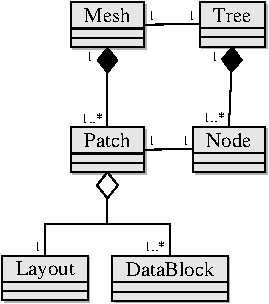
\includegraphics{uml/amr.ps}}

%=======================================================================
\section{Method}
%=======================================================================

Modularized hyperbolic, elliptic, or local physics algorithms,
analysis, and visualization

%=======================================================================
\section{Monitor}
%=======================================================================

User interface to monitor the status of a running simulation

%=======================================================================
\section{Parallel}
%=======================================================================

Low-level functions for facilitating data distribution, communication,
and load balancing

%=======================================================================
\section{Parameters}
%=======================================================================

Input, parse, store, and access run-time parameters

%=======================================================================
\section{Particles}
%=======================================================================

Efficiently represent groups of distributed particles

%=======================================================================
\section{Performance}
%=======================================================================

Measure, and provide functions to access, run-time performance

%=======================================================================
\section{Portal}
%=======================================================================

Interface with other applications, including querying state, modifying
parameters, and post-visualization

%=======================================================================
\section{Schedule}
%=======================================================================
Schedules Tasks to advance the Simulation in time [was Control]

%=======================================================================
\section{Simulation}
%=======================================================================

Specifies the problem(s) to run

%=======================================================================
\section{Task}
%=======================================================================

Encapsulates Methods and data on an Array for a single process /
thread

%=======================================================================
\section{Test}
%=======================================================================

%=======================================================================
\section{User}
%=======================================================================

\centerline{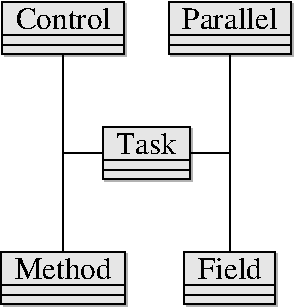
\includegraphics{uml/task.ps}}

%=======================================================================
\chapter{Process View}
%=======================================================================

%=======================================================================
\chapter{Implementation View}
%=======================================================================

%=======================================================================
\chapter{Deployment View}
%=======================================================================


\end{document}

%==================================================================
